~~~~Suppose we generate a data based on the model as show in Figure 4.1. This model is the "Bayesian network model of Asia Data Set by Lauritzen and Spiegelhalter" to be introduced in the next chapter.

\begin{figure}[t]
	\centering
	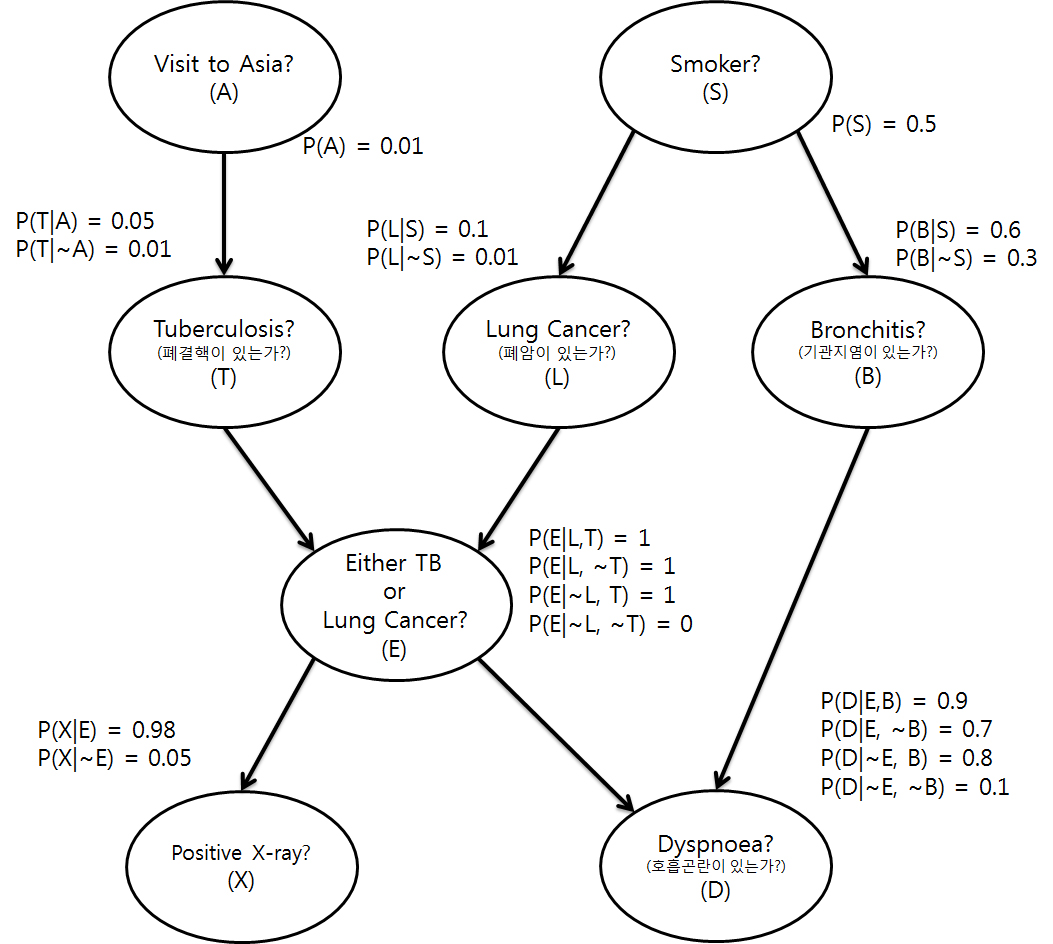
\includegraphics[height=250pt]{images/Real_Asia}
	\caption{BN model of Asia Data Set by Lauritzen and Spiegelhalter}
\end{figure}

It makes Arcs, input$\_$Probs, node$\_$names as follows:

\begin{center}\rule[0.5ex]{0.9\columnwidth}{1pt}\end{center}

R$>$ arcs = rbind(

		~~~~~~~~$\#$	A	S	T	L	B	E	X	D
		
		~~~~~~~~c(0,	0,	1,	0,	0,	0,	0,	0),	$\#$A
		
		~~~~~~~~c(0,	0,	0,	1,	1,	0,	0,	0),	$\#$S
		
		~~~~~~~~c(0,	0,	0,	0,	0,	1,	0,	0),	$\#$T
		
		~~~~~~~~c(0,	0,	0,	0,	0,	1,	0,	0),	$\#$L
		
		~~~~~~~~c(0,	0,	0,	0,	0,	0,	0,	1),	$\#$B
		
		~~~~~~~~c(0,	0,	0,	0,	0,	0,	1,	1),	$\#$E
		
		~~~~~~~~c(0,	0,	0,	0,	0,	0,	0,	0),	$\#$X
		
		~~~~~~~~c(0,	0,	0,	0,	0,	0,	0,	0))	$\#$D
		
R$>$ arc$\_$name = c("A", "S", "T", "L", "B", "E", "X", "D")

R$>$ Probs = list(

	~c(0.01),						$\# P(A)$
	
	~c(0.5), 						$\# P(S)$
	
	~c(0.05, 0.01),				$\# P(T|A), P(T|\sim A)$
	
	~c(0.1, 0.01),				$\# P(L|S), P(L|\sim S)$
	
	~c(0.6, 0.3),					$\# P(B|S), P(B|\sim S)$
	
	~c(1, 1, 1, 0),				$\# P(E|T,L), P(E|\sim T,L), P(E|T,\sim L), P(E|\sim T,\sim L)$
	
	~c(0.98, 0.05),				$\# P(X|E), P(X|\sim E)$

	~$\# P(D|B,E), P(D|\sim B,E), P(D|B,\sim E), P(D|\sim B,\sim E)$
	
	~c(0.9, 0.7, 0.8, 0.1))

\begin{center}\rule[0.5ex]{0.9\columnwidth}{1pt}\end{center}

Suppose the sample size is 1000. If you type objects and sample size into BN$\_$Data$\_$Generator, then the data is generated.

\begin{center}\rule[0.5ex]{0.9\columnwidth}{1pt}\end{center}

R$>$ n = 1000
 
R$>$ res = BN$\_$Data$\_$Generator(arcs, Probs, n, arc$\_$name)

R$>$ data = res$\$$data

R$>$ head(data)

~~~~~~A S T L B E X D
  
~~~~1 N N N N N N N N

~~~~2 N Y N N Y N N Y

~~~~3 N N N N N N N N

~~~~4 N Y N N N N N N

~~~~5 N N N N Y N N N

~~~~6 N Y N N Y N N Y

R$>$ dim(data)

~~~~[1] 1000    8

\begin{center}\rule[0.5ex]{0.9\columnwidth}{1pt}\end{center}

\begin{figure}[h]
	\centering
	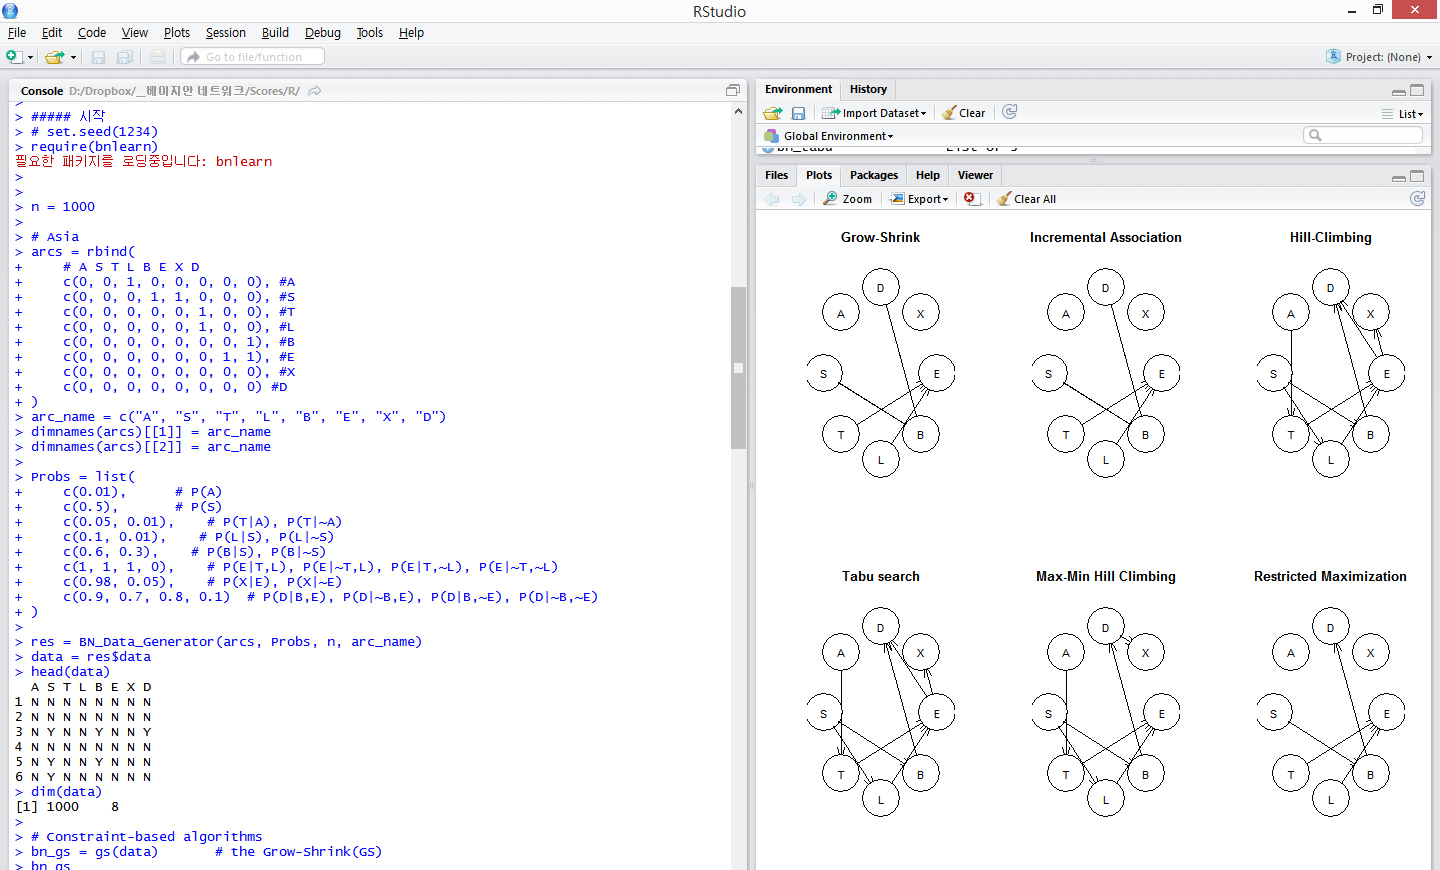
\includegraphics[height=250pt]{images/image23}
	\caption{After make a data, execution results by bnlearn}
\end{figure}